\chapter{牛頓宇宙學與弗里德曼方程}

上次我們談到了空間的度規。接下來要問的是動力學：尺度因子如何隨時間變化？我們先談一點幾何，再談牛頓宇宙學。這裡還不會從廣義相對論推導弗里德曼方程，而是從牛頓方程推導。

\section{均勻性、各向同性與隨時間變化的度規}

均勻性與各向同性是基本假設。如果宇宙均勻且各向同性，並且隨時間演化，那麼哈伯定律就一直成立。在任一固定時刻，退行速度與距離成正比，
\begin{equation}
v = H(t)\,d.
\end{equation}
這種正比關係是線性的。保持不變的不是時間，而是空間：在給定時刻，各處都適用同一個比例因子。

\begin{classroomqa}
\audiencequestion{你的意思是線性正比嗎？}\lecturetimestamp{00:02:06}
\lecturerresponse{是的。在固定時刻，退行速度與距離成線性正比。比例因子就是哈伯常數。一般而言，它會隨時間變化，但不會隨空間位置改變。}
\end{classroomqa}

所以「``哈伯常數''」這個說法容易引起誤解。它對空間位置而言是常數，對時間而言卻不是。

接下來自然會問：如果空間在膨脹，為什麼米尺也不跟著膨脹？答案是，把米尺結合在一起的力，遠強於原子尺度上任何與宇宙膨脹相關的效應。受束縛的物體仍維持束縛狀態。膨脹的是彼此距離足夠遠、互相束縛不強的物體之間的距離，例如相距甚遠的星系。

\begin{classroomqa}
\audiencequestion{測量用的尺也在膨脹，這會不會造成問題？}\lecturetimestamp{00:04:00}
\lecturerresponse{不會。測量用的尺並沒有膨脹，膨脹的是座標。把米尺結合在一起的力遠強於膨脹造成的效應，因此一般受束縛的物體不會隨著背景膨脹。相距足夠遠的星系確實會彼此分離，但米尺不會。}
\end{classroomqa}

甚至可以設想原子之間多了一點微弱的排斥效應，但這仍不足以把尺扯開。它只會稍微改變平衡間距，就像一點額外的拉力會稍微改變剛性彈簧的平衡位置。

\begin{classroomqa}
\audiencequestion{不過，你不能把它建模成作用在點與點之間的力，對嗎？否則它就會造成加速度。}\lecturetimestamp{00:05:29}
\lecturerresponse{可以設想原子之間存在一種微弱的額外作用力，但若它遠小於束縛力，就只會稍微改變平衡位置。單靠膨脹本身，不會產生一般的力定律。某些膨脹形式可以用力來建模，例如加速膨脹，但那是之後才要討論的問題。}
\end{classroomqa}

因此，適用的座標是嵌入在膨脹物質分布中的座標。沒有額外本動的星系，其座標值保持不變。隨時間改變的是座標間距與以公尺量度的物理距離之間的關係；這種關係由尺度因子\(a(t)\)表示。

在平坦空間中，空間度規可以寫成
\begin{equation}
ds^2 = a(t)^2\left(dx^2+dy^2+dz^2\right).
\end{equation}
這裡的\(a\)表示相隔一個單位座標距離的相鄰點之間的實際距離，以公尺為單位。如果宇宙膨脹，\(a\)就會隨時間變化。

要推廣到時空，可以從狹義相對論的形式出發
\begin{equation}
d\tau^2 = dt^2 - ds^2,
\end{equation}
並代入空間度規，得到
\begin{equation}
d\tau^2 = dt^2 - a(t)^2\left(dx^2+dy^2+dz^2\right).
\end{equation}
這些係數不隨空間位置改變，只隨時間變化。這就是均勻性在度規語言中的表述。對角度規的形式如下：
\begin{equation}
g_{\mu\nu}=\mathrm{diag}\!\left(1,-a(t)^2,-a(t)^2,-a(t)^2\right).
\end{equation}
\editorialnote{此處寫出的完整對角矩陣，依據的是00:14:33附近對度規張量的口頭描述。黑板畫面清楚顯示了線元素，但矩陣本身無法完整辨讀。}

沒有非對角項：沒有\(dx\,dy\)，沒有\(dx\,dt\)，也沒有其他混合項。這個度規幾乎和閔考斯基時空的度規一樣簡單。特別之處在於，空間尺度與時間之間的關係本身也隨時間變化。

\begin{figure}
\centering
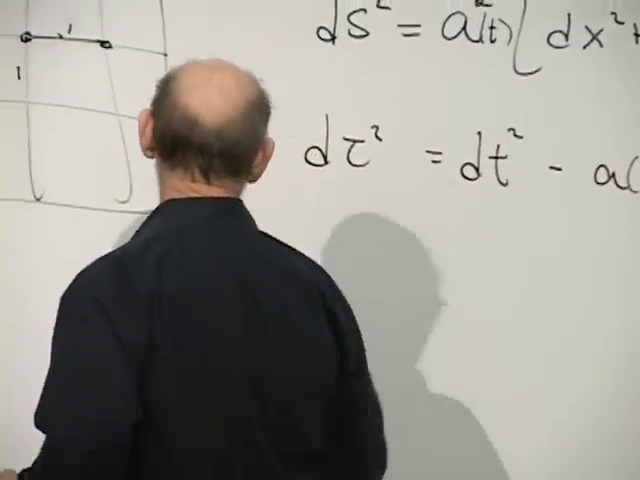
\includegraphics[width=0.62\textwidth]{lecture_02_figure_02.png}
\caption{共動座標網格示意圖，以及含時尺度因子的時空間隔。}
\end{figure}

圖示說明了重點。Alice 和 Bob 在共動座標中始終相隔一個單位，但隨時間經過，這一個座標單位所代表的公尺數愈來愈多。如果過去某個時刻的\(a(t)\)等於零，那麼所有物理距離都會是零，一切都會擠在一起。這就是為什麼\(a\to 0\)對應到無限密度。隨著\(a\)增大，宇宙會愈來愈稀薄。

這種度規形式並不適用於所有參考系；它適用於隨星系運動的參考系。

\begin{classroomqa}
\audiencequestion{那個方程裡的小\(t\)、\(a(t)\)，它的\(t\)是指什麼？}\lecturetimestamp{00:19:19}
\lecturerresponse{它是隨星系運動的時鐘所量到的時間。想像有一座宇宙時鐘工廠，製造出相同的時鐘，再把它們交給星系攜帶。在這個參考系中，時間變數正是這些時鐘所量到的時間。沿著星系的世界線，固有時等於這個座標時間。}
\end{classroomqa}

確實，沿著共動星系的世界線，
\begin{equation}
dx=dy=dz=0,
\end{equation}
所以
\begin{equation}
d\tau^2 = dt^2,
\end{equation}
因此
\begin{equation}
dt=d\tau.
\end{equation}

\begin{classroomqa}
\audiencequestion{有沒有能讓這種度規形式保持不變的變換？}\lecturetimestamp{00:23:08}
\lecturerresponse{旋轉可以，因為\(dx^2+dy^2+dz^2\)在旋轉下保持不變。但洛侖茲推進不會保留這種形式。物質本身選出了隨星系運動的參考系；在其他參考系中，宇宙看起來就不會是各向同性的。}
\end{classroomqa}

\section{重力場中的拋射體}

在把牛頓定律應用於整個宇宙之前，先回頭看一個較簡單的問題會有幫助：一個大質量\(M\)、一個小得多的質量\(m\)，以及一個初始的向外衝量。衝量作用之後，小質量只是在重力場中運動，依照牛頓定律演化。

在宇宙學的討論中，重要的不是完整的軌道問題，而是能量守恆。動能為
\begin{equation}
\frac{1}{2}mv^2.
\end{equation}

\begin{figure}
\centering
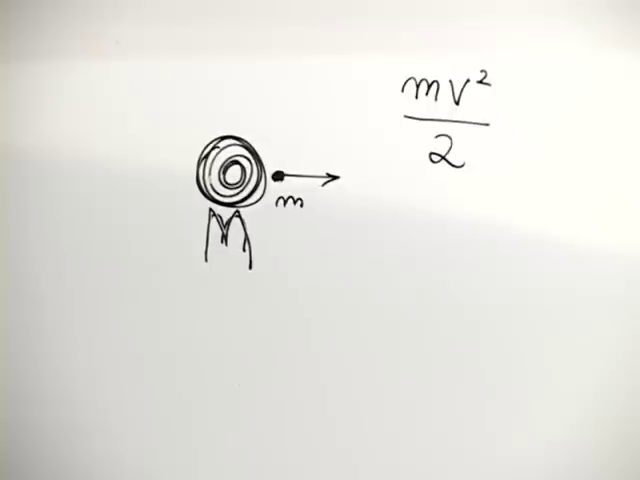
\includegraphics[width=0.42\textwidth]{lecture_02_figure_03.png}
\caption{向外運動的試驗質量與動能項\(\frac{1}{2}mv^2\)。}
\end{figure}

重力位能包含兩個質量的乘積、牛頓常數，以及分母中的一階距離。黑板上這些因子的排列順序是\(mMG/D\)，因此這裡最好沿用該順序：
\begin{equation}
-\frac{mMG}{D}.
\end{equation}
所以總能量為
\begin{equation}
\frac{1}{2}mv^2-\frac{mMG}{D}.
\end{equation}
能量守恆只表示，對正在討論的這個粒子而言，這個量不隨時間改變。不同粒子的能量可以不同。

\begin{figure}
\centering
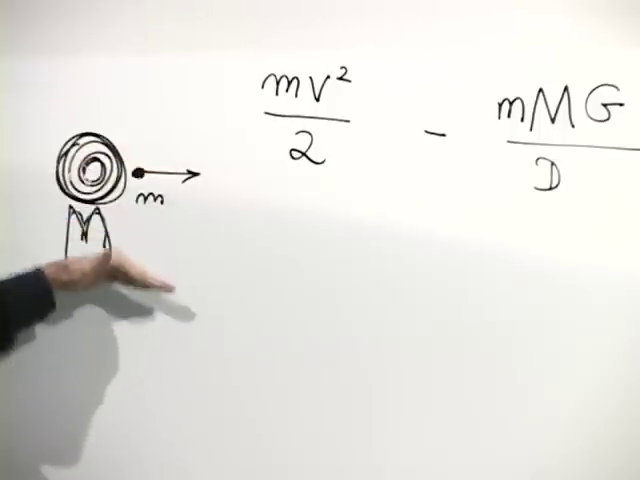
\includegraphics[width=0.62\textwidth]{lecture_02_figure_04.png}
\caption{徑向運動的試驗質量之牛頓總能量：動能減去重力位能。}
\end{figure}

負號很重要。重力位能是負的，因為重力具有吸引性。粒子愈靠近，位能就愈負；粒子移得愈遠，位能就愈不負。

\begin{classroomqa}
\audiencequestion{位能是隨距離增加而上升，不是下降嗎？}\lecturetimestamp{00:34:13}
\lecturerresponse{是的。先不管常數，看看\(1/D\)和\(-1/D\)的圖形。力會使物體朝位能降低的方向運動。因此，吸引力對應到倒過來的曲線\(-1/D\)；位能會隨距離增加而上升，粒子向內移動時則變得更負。}
\end{classroomqa}

\begin{figure}
\centering
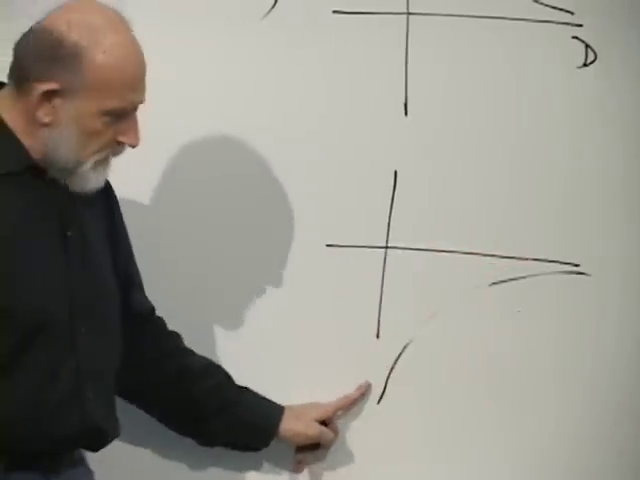
\includegraphics[width=0.46\textwidth]{lecture_02_figure_05.png}
\caption{比較\(1/D\)與\(-1/D\)的定性圖形，以說明重力位能的正負號。}
\end{figure}

\section{逃逸速度}

現在來分類各種可能性。能量可以是正、負或零，只有這三種情況。

\begin{itemize}
\item 能量為負時，粒子是受束縛的。若以太小的速度把它向上拋，它會上升、減速、折返，然後落回來。
\item 能量為正時，粒子會逃逸。重力起初會使它減速，但減速不足以讓它停下來；最後它會以非零的漸近向外速度遠離。
\item 能量恰好為零時，粒子正好達到逃逸速度。這是能否逃逸的臨界情況。
\end{itemize}

初始速度夠小時，一開始就是位能項占優勢，因此總能量為負。

\begin{figure}
\centering
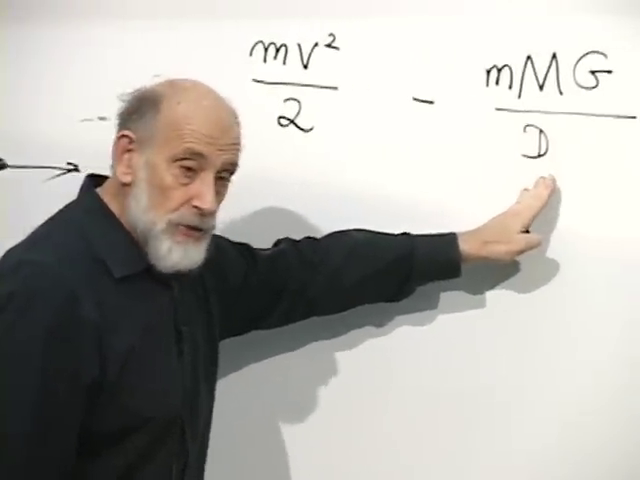
\includegraphics[width=0.62\textwidth]{lecture_02_figure_06.png}
\caption{向外速率較小時，負的位能項在總能量中占優勢。}
\end{figure}

在零能量的情況下，距離持續增加，但速率持續減小。粒子不可能在有限時間內停下來；如果真的停下來，它就會掉回去。因此距離沒有上限，而速度趨近於零。

這就是對宇宙學有用的直接類比。宇宙也可能有相同的演化方式。若初始向外的哈伯流夠強，所有物體都會彼此遠離；若不夠強，重力就會勝出，宇宙將發生大崩塌。兩者之間還有一個臨界情況，恰好類似逃逸速度。

\section{牛頓定理}

之所以能將宇宙學問題化簡，是因為平方反比定律適用的牛頓定理。

如果物質以某個中心為對稱中心呈球對稱分布，那麼對分布外的粒子而言，重力作用恰好等同於全部質量集中在中心。但這個定理更進一步：如果粒子位於分布內部，只有半徑較小處的質量會產生作用；半徑較大處的質量不會產生淨力。

這個定理最簡潔的情形是薄殼。完美的球殼對殼內任何位置的粒子都不產生重力，即使粒子不在中心也是如此。乍看之下或許令人驚訝，但這確實是\(1/r^2\)定律的結果。

\begin{classroomqa}
\audiencequestion{你剛才舉的例子裡，粒子穿越邊界時，力似乎不連續；這點是不是有些令人驚訝？}\lecturetimestamp{00:48:19}
\lecturerresponse{是的。對理想的無限薄球殼來說，這確實令人驚訝，而且是\(1/r^2\)力定律特有的結果。真實的球殼有厚度，因此力的變化會平滑一些；但理想薄殼的這個明確結果，正是牛頓定理令人驚奇的性質。}
\end{classroomqa}

用一幅圖來想像，這個定理就比較容易理解。把點質量換成點狀水源。在三維空間中，向外的流量會按\(1/r^2\)遞減。把這種水源連續地分布在球殼上。球殼外的流動，恰好就像所有水源都集中在中心；球殼內則不會有淨流動，因為中心沒有水源。重力定理背後也是相同的結構。

這裡的重點不是重新推導定理，而是運用它。

\section{將均勻宇宙化為單體問題}

現在回到宇宙學。取宇宙中的一小塊區域，其中充滿均勻分布的星系。如果方便，也可以把自己放在中心。這只是為了方便；任何人都可以說自己位於中心，而推導出的方程都應該相同。

選取一個位於\(x\)軸上、共動座標為\(x\)的星系。由於宇宙具有各向同性，選哪條軸都無關緊要。以\(x=0\)為球心，畫一個通過該星系的球面。根據牛頓定理，作用在該星系上的力，恰好等同於球內所有質量都集中在球心時的情況；球外的物質則沒有貢獻。

這個球會隨星系一起膨脹。它始終包含相同的星系，因此總質量也不變，雖然它的物理半徑會隨時間改變。

因此，該星系的運動遵循與拋射體相同類型的能量方程：
\begin{equation}
\frac{1}{2}mv^2-\frac{mMG}{D}=\text{constant}.
\end{equation}
這裡的\(M\)現在指膨脹球體內的質量，而不是前面簡單例子中的中心質量。接著，將方程乘以\(2\)並除以\(m\)，即可簡化代數式。常數除以\(m\)仍然只是常數，因此可以寫成
\begin{equation}
v^2-\frac{2MG}{D}=\text{constant}.
\end{equation}
同樣地，「``常數''」是指對這個特定星系而言，該量不隨時間改變。

現在把這個結果與尺度因子連結起來。到該星系的物理距離為
\begin{equation}
D=ax,
\end{equation}
因為\(x\)是固定的共動座標。它的速度為
\begin{equation}
v=\dot D=\dot a\,x.
\end{equation}

球內的質量等於密度乘以體積。若\(\rho\)表示質量密度，則
\begin{equation}
M=\frac{4\pi}{3}\rho D^3=\frac{4\pi}{3}\rho a^3x^3.
\end{equation}
代入能量方程可得
\begin{equation}
\dot a^2x^2-\frac{2G}{ax}\left(\frac{4\pi}{3}\rho a^3x^3\right)=\text{constant},
\end{equation}
也就是
\begin{equation}
\dot a^2x^2-\frac{8\pi G}{3}\rho a^2x^2=\text{constant}.
\end{equation}

左側兩項都正比於\(x^2\)，而左側其他量在各處都相同。因此右側也必須正比於\(x^2\)。這和稱它為常數並不矛盾：對每個固定的\(x\)而言，它不隨時間變化，但從一個星系到另一個星系，它仍可能隨\(x^2\)改變。這很合理，因為距離較遠的星系運動得比較快。

因此，約去共同因子\(x^2\)。剩下的常數現在不隨時間或空間改變。依照歷史上慣用的方式，把它寫成\(-k\)：
\begin{equation}
\dot a^2-\frac{8\pi G}{3}\rho a^2=-k.
\end{equation}
再除以\(a^2\)，得到
\begin{equation}
\left(\frac{\dot a}{a}\right)^2=\frac{8\pi G}{3}\rho-\frac{k}{a^2}.
\end{equation}

這就是著名的弗里德曼－羅伯遜－沃克方程，不過講課時也提到，這其實就是弗里德曼方程。符號的選法沿襲自歷史。寫成\(-k\)不表示\(k\)必須為正；\(k\)可以為正、為負或為零。在光速設為\(1\)的單位制中，\(k\)是無因次量。

\section{密度與物質主導的方程}

接下來自然要問：\(\rho\)是什麼？它不是常數。宇宙膨脹時，密度會降低。

要表示這種變化，可以在座標空間取一個單位立方體：沿\(x\)、\(y\)和\(z\)方向的邊長各為一個單位。由於立方體隨座標一起膨脹，裡面始終是相同的星系。因此，這個座標立方體內的質量固定不變。

\editorialnote{講課中在不同階段重複使用符號\(M\)。這裡以\(M_{\Box}\)表示單位座標立方體內的質量，藉此和前面提到的中心質量及球內質量區分。}

立方體的物理邊長是\(a\)，所以物理體積為\(a^3\)。因此
\begin{equation}
\rho=\frac{M_{\Box}}{a^3}.
\end{equation}
這是物質主導的情況：方程右側只包含普通非相對論性物質的密度。

\begin{classroomqa}
\audiencequestion{根據這個方程，哈伯常數是\(\rho\)的函數，所以它不是常數。}\lecturetimestamp{01:19:21}
\lecturerresponse{正是如此。哈伯常數不是常數。它取決於密度，而密度會隨時間變化。講課時甚至開玩笑說，期末考只要出一題就夠了：哈伯常數是常數嗎？}
\end{classroomqa}

將\(\rho=M_{\Box}/a^3\)代入弗里德曼方程，得到
\begin{equation}
\left(\frac{\dot a}{a}\right)^2=\frac{8\pi G M_{\Box}}{3a^3}-\frac{k}{a^2}.
\end{equation}

現在可以看出有哪些任意選擇：需要知道單位座標立方體內的質量，以及\(k\)的值。\(k\)的三種可能符號，分別對應拋射體問題中的三種能量情況。

\begin{itemize}
\item 若\(-k>0\)，能量相當於高於逃逸速度，宇宙會永遠膨脹。
\item 若\(-k<0\)，重力終將勝出，宇宙會重新坍縮。
\item 若\(k=0\)，宇宙恰好處於逃逸速度的臨界情況。
\end{itemize}

\begin{classroomqa}
\audiencequestion{若\(k=0\)呢？那麼兩個星系之間的速度會趨近於零嗎？}\lecturetimestamp{01:21:12}
\lecturerresponse{是的。在臨界情況下，速度會趨近於零，但距離仍然沒有上限。星系持續分離，只是速度愈來愈慢。如果它們真的在有限時間內停下來，就會掉回去。}
\end{classroomqa}

\section{臨界情況 \(k=0\)}

現在選擇最簡單的情況，也就是\(k=0\)。這正是逃逸速度的臨界情況；它之所以簡單，只是因為數學比較簡單。方程變成
\begin{equation}
\left(\frac{\dot a}{a}\right)^2=\frac{8\pi G M_{\Box}}{3a^3}.
\end{equation}

右側恆為正，從不等於零。因此\(\dot a/a\)不可能變為零。在這種情況下，宇宙不可能掉頭；它只能一直膨脹或一直收縮。這裡選擇膨脹分支。

現在猜測解具有冪次律的形式：
\begin{equation}
a(t)=ct^p.
\end{equation}
於是
\begin{equation}
\dot a = cp\,t^{p-1},
\end{equation}
因此
\begin{equation}
\frac{\dot a}{a}=\frac{p}{t}.
\end{equation}
代入微分方程，得到
\begin{equation}
\frac{p^2}{t^2}=\frac{8\pi G M_{\Box}}{3c^3t^{3p}}.
\end{equation}
要讓\(t\)的冪次相符，必須有
\begin{equation}
3p=2.
\end{equation}
所以
\begin{equation}
p=\frac{2}{3}.
\end{equation}
接著，常數必須滿足
\begin{equation}
\frac{4}{9}=\frac{8\pi G M_{\Box}}{3c^3},
\end{equation}
因此
\begin{equation}
c^3=6\pi G M_{\Box}.
\end{equation}
所以
\begin{equation}
a(t)=\left(6\pi G M_{\Box}\right)^{1/3}t^{2/3}.
\end{equation}

仍可能有一個加法形式的時間平移；把\(t\)換成\(t-t_0\)就能將它吸收。選擇時間原點，使\(t=0\)時\(a=0\)，剩下的常數便消失。

所以宇宙的膨脹尺度與時間的三分之二次方成正比，
\begin{equation}
a(t)\propto t^{2/3}.
\end{equation}
膨脹並非隨時間線性增加。線性成長相當於不加速的運動；這裡的膨脹則逐漸減慢。

若把公式往回推到\(t=0\)，尺度因子會降為零，密度則發散。\(a=0\)這種情況極端得難以想像。我們不知道物質在密度極高時會變成什麼樣子。真正的重點是，在宇宙早期的某個階段，一切都極度擁擠，原子、原子核和夸克全都擠在一起，處於極端高密度的狀態。

\section{哈伯常數與宇宙年齡}

在臨界模型中，
\begin{equation}
H(t)=\frac{\dot a}{a}=\frac{2}{3t}.
\end{equation}
所以哈伯常數約等於宇宙年齡的倒數：
\begin{equation}
t=\frac{2}{3H}.
\end{equation}
這是這項計算的一個主要成果。測量今天的哈伯常數，就能估算宇宙的年齡，至少可以回溯到牛頓模型不再適用之處。

引用的宇宙年齡約為\(13\)到\(14\)億年。文中也指出，\(k=0\)在觀測上相當符合實際：以文中引用的精度而言，尚未發現與\(k=0\)有顯著差異。

\begin{classroomqa}
\audiencequestion{我有點不太清楚\(M\)和\(a\)代表什麼。}\lecturetimestamp{01:39:16}
\lecturerresponse{兩者都帶有座標網格選擇所造成的任意性。改變基準立方體，其中的物質量會跟著改變，尺度因子的數值也會改變。具有物理意義的是密度\(M/a^3\)，或等價地，像\(a/M^{1/3}\)這樣不受網格選擇影響的組合。在\(k=0\)的解中，乘在\(t^{2/3}\)前面的未知常數會在\(\dot a/a\)中消去，因此年齡關係\(t=2/3H\)不取決於基準立方體內的質量。}
\end{classroomqa}

從解可以直接看出這個消去過程。若
\begin{equation}
a(t)=Ct^{2/3},
\end{equation}
則
\begin{equation}
\dot a=\frac{2}{3}Ct^{-1/3},
\end{equation}
因此
\begin{equation}
\frac{\dot a}{a}=\frac{2}{3t}.
\end{equation}
常數\(C\)完全消去。

\section{牛頓推導為何成立}

講到後面，問題就變成：為什麼牛頓推導能和相對論推導如此一致？

\begin{classroomqa}
\audiencequestion{這一切似乎都以宇宙為開放宇宙為前提。}\lecturetimestamp{01:45:44}
\lecturerresponse{目前的推導仍是牛頓式的，而牛頓物理意味著空間是平直的。至於 \(k\) 在空間幾何上的意義，留待下一講再說。屆時，\(k=0\)將對應平直空間，而其他符號則與彎曲的空間幾何相關。}
\end{classroomqa}

\begin{classroomqa}
\audiencequestion{很久以前，米尺的長度會不會取決於\(a\)？}\lecturetimestamp{01:47:53}
\lecturerresponse{在非常早期，物質會擁擠到分開的米尺根本無法存在；在那之前，它們也會被擠壓在一起。講課時也提醒我們，相對論不允許物體真正剛性：如果物體完全剛性，在一側推它，訊號就會瞬間傳到另一側，速度超過光速。}
\end{classroomqa}

\begin{classroomqa}
\audiencequestion{你認為牛頓方程和相對論方程為什麼會有這種巧合？}\lecturetimestamp{01:49:03}
\lecturerresponse{因為牛頓力學只用在足夠小的區域內。只要這個區域相較於整個宇宙的曲率半徑夠小，而且其中局部的哈伯速度遠低於光速，牛頓力學就是很好的近似。講課時把這件事比作研究地球上的草如何生長：不必考慮整個地球的曲率，也能理解局部的生長過程。}
\end{classroomqa}

這就是局部區域的推理方式。牛頓力學首先假設空間曲率對眼前的問題不重要，其次假設局部沒有任何物體以接近光速運動。在宇宙學中，這表示所選區域必須大到足以均勻，同時又要小到可以忽略曲率效應，並使哈伯速度維持在非相對論範圍內。

有了這個理解，牛頓計算就不是偶然得到的結果，而是某個方程在局部的近似；那個方程也可以用相對論的形式來表達。把曲率項移到左側，弗里德曼方程就變成
\begin{equation}
\left(\frac{\dot a}{a}\right)^2+\frac{k}{a^2}=\frac{8\pi G}{3}\rho.
\end{equation}
左側是幾何量，包含尺度因子，以及下一講會談到的空間曲率；右側則是能量密度。這正是廣義相對論所預期的方程形式。

下一講將討論曲率本身、愛因斯坦方程，以及相對論推導與牛頓推導之間的關係。
